\documentclass[10pt, english, makeidx, a4paper, titlepage, oneside]{report}
% Geometry package
\usepackage[a4paper,width=150mm,top=30mm,bottom=25mm]{geometry}
\geometry{hmarginratio=1:1}

% General packages
\usepackage[utf8]{inputenc}
%\usepackage[italian]{babel}
\usepackage{hyperref}
\hypersetup{colorlinks=true}
\hypersetup{linkcolor=black}
\usepackage{siunitx}	% SI measurement units
\usepackage{amsmath}

% Graphics packages
\usepackage{xcolor}
\usepackage{multicol}
\usepackage{graphicx}
\usepackage{float}
\usepackage{hhline}
\usepackage{todonotes}
\usepackage{algorithmic}
\usepackage{subcaption}
\graphicspath{{images/}}

% Custom commands
%\newcommand{\rshift}{\ \texttt{>>}\ }
%\newcommand{\lshift}{\ \texttt{<<}\ }
% TITLE
\usepackage{tikz}
\usetikzlibrary{arrows,shapes,automata,petri,positioning,calc}

\usepackage{mdframed}
\usepackage{listings}
%\definecolor{codeBackground}{RGB}{250, 250, 250}
\definecolor{codeColor}{RGB}{50, 50, 50}
\definecolor{codeComment}{RGB}{90, 90, 90}
\definecolor{codeString}{RGB}{50, 175, 50}

\lstdefinestyle{lstStyle}{
    %backgroundcolor=\color{codeBackground},
    basicstyle=\ttfamily\footnotesize\linespread{0}\color{codeColor},
    commentstyle=\ttfamily\footnotesize\color{codeComment},
    keywordstyle=\bf\color{orange},
    stringstyle=\color{codeString},
    frame=tlbr,
    numbers=left,
    breaklines=true,
    showstringspaces=false,
    tabsize=2
}
\lstset{style=lstStyle}

\title{
	{\Huge \textbf{Politecnico di Torino}}\\ \ \\
	{\Huge Integrated Systems Architectures} \\
	{\large Report for Lab 2}\\
	{\small \url{https://github.com/levnikolaevicmiskyn/ISA/tree/main/lab2}} \\ \ \\
	{\includegraphics[width=0.5\textwidth] {Politecnico_di_Torino.png}}
}
\author{
    {\Large \textsc{Group 12}}\\ \ \\
	Antonio Carlucci 276128\\
	Gabriele Perrone 269089\\
	Alessandro Scisca 276032
}
\date{} % Do not insert date
% START OF THE DOCUMENT
\begin{document}
\maketitle
\tableofcontents
\hypersetup{linkcolor=blue}
\newpage

\chapter{Pipelining the multiplier}
\section{Pipelining}
The command \texttt{set\_implementation} can be useful to force Synopsys to use a particular architecture when synthesizing a given component. In our case, the multiplier can be implemented in several ways differing in how partial products are summed. When no directive is given, the zero clock period constraint will drive the algorithm to resort to pparch, the fastest architecture among those analyzed here. The solution denoted as CSA, based on a carry-save adders tree, seems to be less advantageous in both performance and area. 
\begin{table}[h]
	\centering
	\begin{tabular}{|l|l|l|l|}\hline
		Architecture & Delay & Area & Combinational area \\\hline
		Unspecified (pparch) & 1.4 & 4122 & 2976 \\\hline
		CSA & 3.9 & 4906 & 3764 \\\hline
		pparch & 1.41 & 4104 & 2961 \\\hline
	\end{tabular}
\caption{Comparison of multiplier architectures}
\end{table}
\section{Fine Grain Pipelining}
In order to further boost the performance of this floating point multiplier, an additional pipeline register has been inserted in the second stage just after the multiplier. In this case, however, it has been explicitly coded instead of relying on the automatic retiming tool.

\autoref{tab:stage2} shows a full comparison of timing and area requirements as the number of pipeline stages increase. The alternative command \texttt{compile\_ultra -retime} has been compared with \texttt{optimize\_registers} for the first case: the latter has proven to be more effective in minimizing delay. Synthesis with additional pipeline registers has been performed using \texttt{optimize\_register}, implicit in the table below.

\begin{table}[htbp]
    \centering
	\begin{tabular}{|r|r|r|r|r|}
	\hline
	                       &\texttt{NPIPE=1} & \texttt{NPIPE=2} & \texttt{NPIPE=4} & \texttt{NPIPE=6}\\\hline
	Delay                   & 0.78             & 0.71             & 0.68             & 0.72 \\\hline
    Area (total)           & 5329             & 5595             & 5793             & 6070 \\\hline
    Area (combinational)   & 3068             & 3039             & 2991             & 2978 \\\hline
	\end{tabular}
	\caption{Critical path delay and area with the hardcoded register in the second stage and a varying \texttt{NPIPE}}
	\label{tab:stage2}
\end{table}
It is possible to see how the delay decreases as more registers are added. This is no longer true for \texttt{NPIPE} = 6: the overhead introduced by the setup, skew and jitter times of the new registers surpasses the advantages given by theoretical pipelining.\\
It is interesting to notice how while the total area increases, the combinational area, instead, steadily decreases. This is possibly due to the fact that the pipelining technique relaxes not only the timing constraints of the combinational logic, but also the power constraints: since the combinational paths are broken into smaller sections, there is less necessity for buffers and also the cells themselves no longer need as much driving strength, thus can also be smaller.

\begin{table}[htbp]
	\centering
	\begin{tabular}{|r|r|r|}
		\hline
								& compile\_ultra 	& optimize\_register \\\hline
		Delay            		& 1.37				& 0.78  \\\hline
		Area (total)        	& 4395 				& 5329   \\\hline
		Area (combinational)	& 3065 				& 3068   \\\hline
	\end{tabular}
	\caption{Critical path delay and area with the hardcoded register in the second stage and a varying \texttt{NPIPE}}
	\label{tab:stage2_opt_vs_ultra}
\end{table}

\paragraph{Critical path delay distribution}
\autoref{fig:hist2} and \autoref{fig:hist6} show how worst path delays tend to accumulate towards the shortest one as the degree of pipelining increases. This is a general pattern seen when applying this technique.
\begin{figure}[htbp]
    \begin{subfigure}{0.5\textwidth}
	   \centering
	   \includegraphics[width=\textwidth]{chapter1/images/npipe2.png}
	   \caption{Worst path distribution with \texttt{NPIPE=2}}
	   \label{fig:hist2}
    \end{subfigure}
    \begin{subfigure}{0.5\textwidth}
        \centering
	    \includegraphics[width=\textwidth]{chapter1/images/npipe6.png}
	    \caption{Worst path distribution with \texttt{NPIPE=6}}
	    \label{fig:hist6}
	\end{subfigure}
\end{figure}


\chapter{Basic Architecture}
\section{Datapath}
The datapath has been derived directly from the DFG from \autoref{fig:iir-dfd}, obtaining the architecture shown in \autoref{fig:datapath-simple}.

\begin{figure}[htbp]
	\centering
	\makebox[\textwidth][c]{
	\includegraphics[width=\textwidth]{./chapter2/images/datapath.png}}
	\caption{IIR filter datapath}
	\label{fig:datapath-simple}
\end{figure}

The specified timing requires input data to be sampled on the same clock cycles where \texttt{VIN} is asserted. For this reason, the input register \texttt{R1} is always enabled. The most convenient solution to carry on operations only when data is actually valid is to place a latch at the output of \texttt{R1}.\\
This is because appending another register instead of a latch will increase the overall latency; while selectively enabling the internal registers complicates their internal structures. Furthermore, the input latch will also act as a power gating circuit, preventing the waste of power in the internal combinatorial nodes when the input samples are not valid.

Overall, the only real commands needed from the control unit are \texttt{en\_latch} and \texttt{clr\_w\_reg}.

\subsection{Accuracy}
Given the results from \autoref{sec:THD}, it is possible to see that $n_b=7$ is enough to meet the requirements. This means that dropping the least significant bit from the input samples (represented on 8 bits) can simplify the internal computations with an acceptable degradation in accuracy.

The previous analysis had been carried using a model where numbers include $n_b-1$ fractional bits (the binary digits with weights $2^{-1}$, $2^{-2}$, ..., $2^{n_b-2}$), therefore it is expectable that allocating 6 fractional bits for all the internal variables in the VHDL implementation will provide enough accuracy.

\subsection{Avoiding overflow}
The C reference model is accurate in predicting the error introduced by truncation, which affects the output of every multiplier block, but it neglects the inability to represent a number larger or equal to 1 in absolute value with the single integer bit available in the standard fixed-point format.\\
An overflow condition may occur in intermediate steps of the computation where the result would require more than one integer bit. In order to determine the right sizing that guarantees the absence of overflow, the maximum value of the intermediate variable $w[n]$ must be determined. Using \autoref{eqn:iir},
\begin{align*}
	w[n] &= \sum_{i=0}^{n} (-a_1)^i x[n-i]
\end{align*}
Hence, assuming $|x[n]|\leq 1$,
\begin{align*}
	|w[n]|\leq
	\sum_{i=0}^{n} |(-a_1)^i x[n-i]| \leq
	\sum_{i=0}^{n} |a_1|^i \leq
	\frac{1}{1-|a_1|} \approx
	1.2
\end{align*}
According to this computation, two integer bits are enough to avoid overflow at the nodes where $w[n]$ is processed within the DFG. As a consequence, the adder and multiplier in the feedback loop in \autoref{lab1:fig:iir-dfd} will operate on inputs with 2 integer bits and 6 fractional bits, as already determined by the previous reasoning on the internal accuracy.\\
As for the operators in the feedforward part, multiplying $w[n]$ and $w[n-1]$ by $b_1$ and $b_2$ will always produce a result lower than 1 in magnitude, for which a single digit to the left of the radix point suffices. Therefore the output of those multipliers is resized to match the same format used by the final adder consisting of 1 integer and 6 fractional bits. The eighth digit, which is always zero, is appended to the final result, thus becoming its LSB, to comply with the specified interface format. A summary of the internal parallelism used throughout the filter is reported in \autoref{lab1:fig:parallelism}.
\begin{figure}[htbp]
	\centering
	\makebox[\textwidth][c]{
	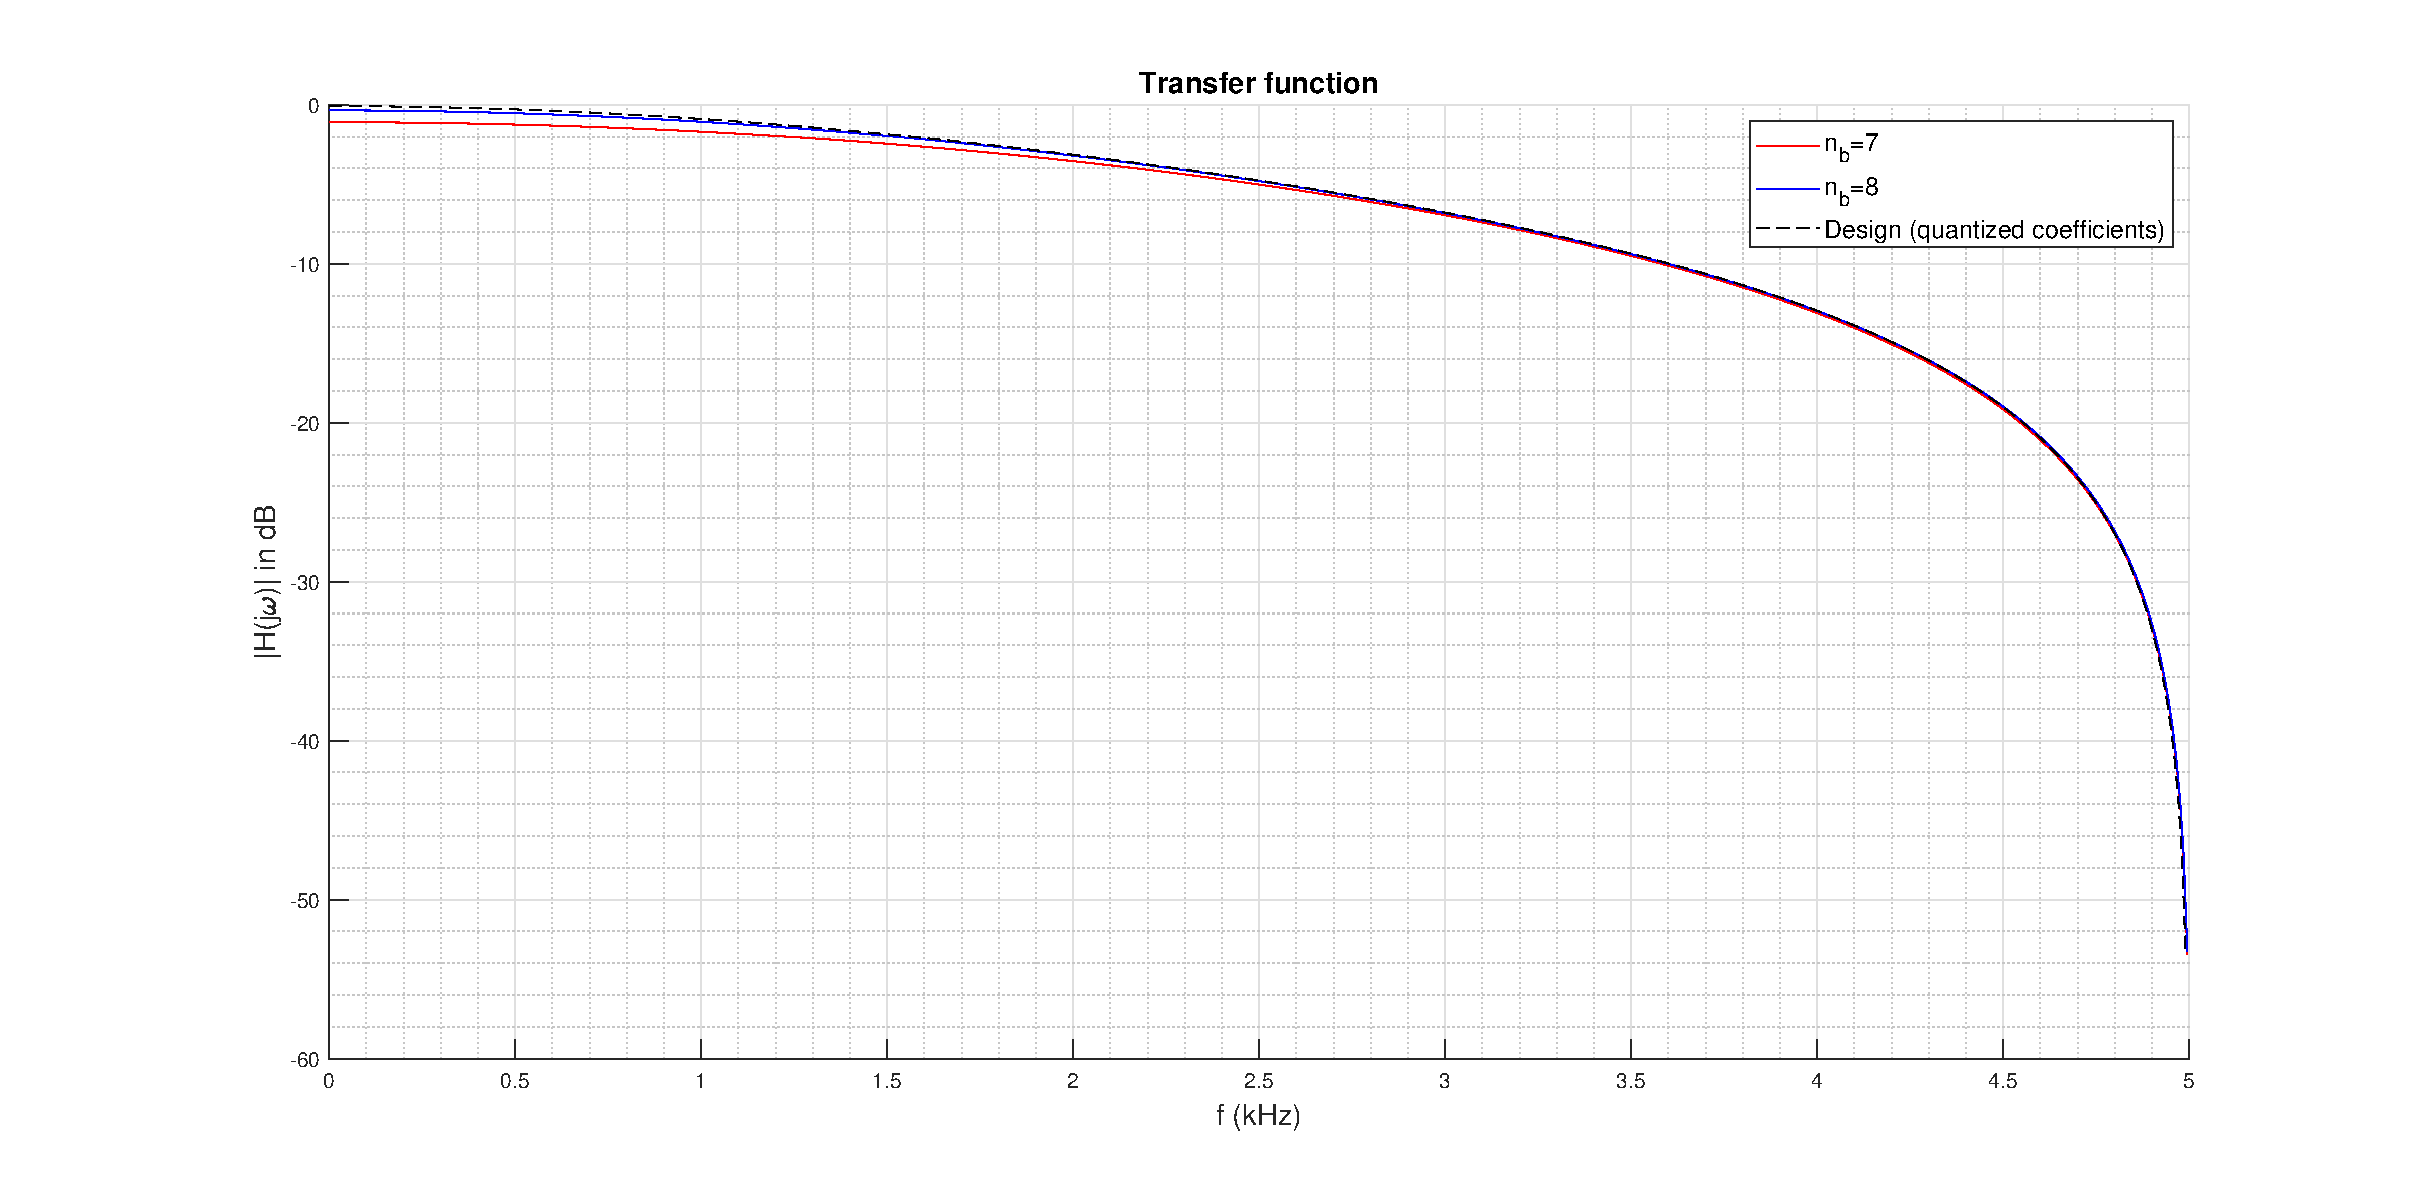
\includegraphics[width=1.4\textwidth]{./chapter1/images/tf_comparison.eps}}
	\caption{Transfer function for a few values of $n_b$}
	\label{fig:tfcomparison}
\end{figure}
\begin{figure}[htbp]
	\centering
	\makebox[\textwidth][c]{
	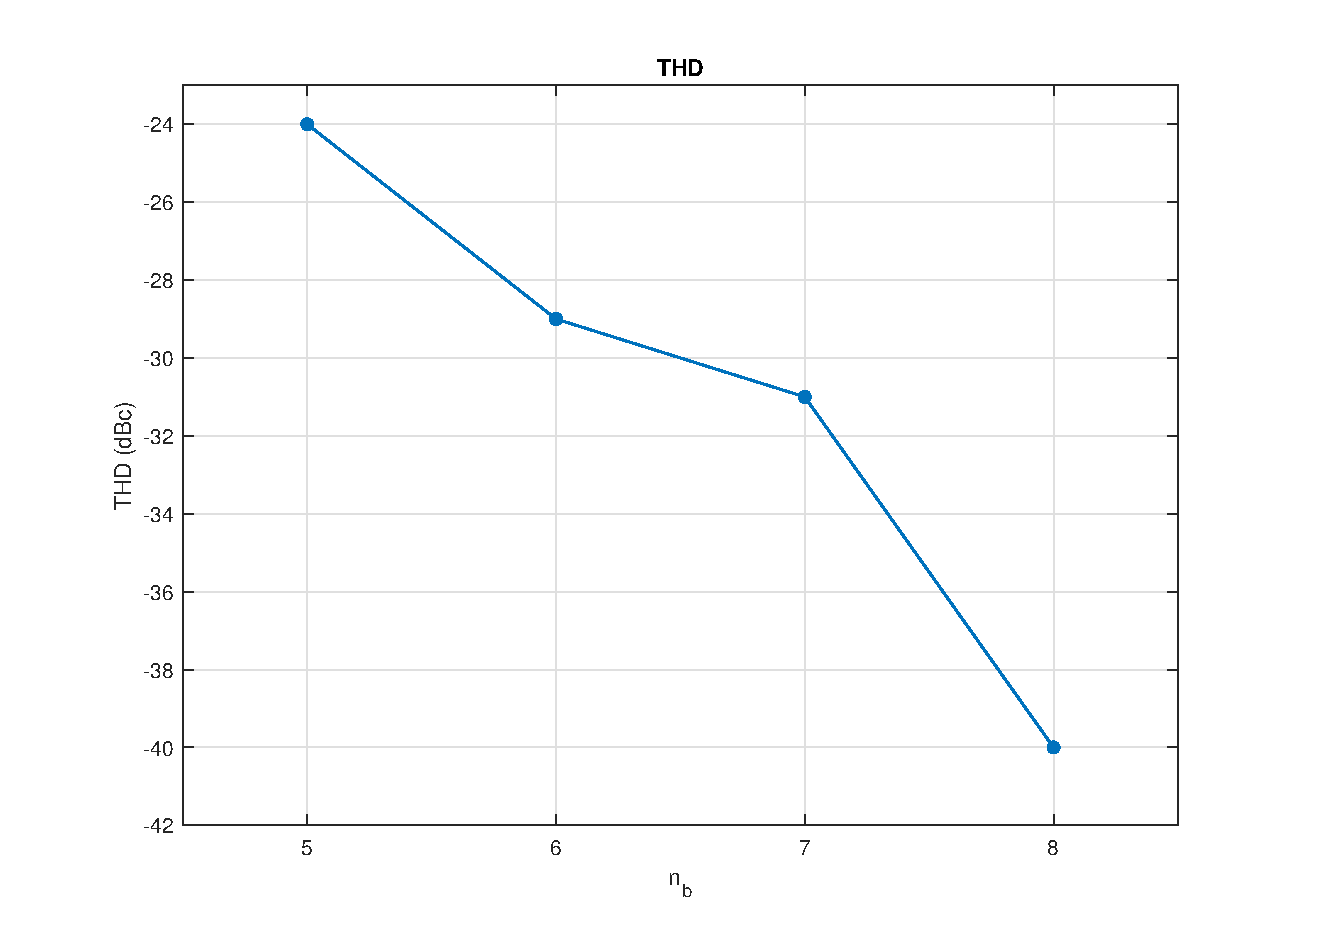
\includegraphics[width=1.4\textwidth]{./chapter1/images/thdplot.eps}}
	\caption{THD as a function of $n_b$}
	\label{fig:thdplot}
\end{figure}

\section{Synthesis}
The final design has been synthesized. The maximum frequency analysis is reported in \autoref{tab:maxtime}. In a second run, the clock period has been set to $4T_{min} = 4.8\,\textrm{ns}$, with the data reported in \autoref{tab:normaltime}.
\begin{table}
	\parbox[t]{0.53\textwidth}{
	\centering
	
\begin{tabular}[t]{|lrr|}  
	\hline
	\textbf{Point}                                                  & \textbf{Incr}   &    \textbf{Path}\\\hline
clock CLK (rise edge)                                 &  0.00     &   0.00\\
clock network delay (ideal)                          &    0.00     &  0.00\\
comp\_dp/w1\_reg[0]/CK                     &    0.00     &   0.00 \\
comp\_dp/w1\_reg[0]/Q                          &  0.10   &     0.10\\ comp\_dp/comp\_m2/a[0]  &0.00    &    0.10\\
comp\_dp/comp\_m2/mult\_31/a[0]  & 0.00     &   0.10       \\
...& &\\
comp\_dp/m2out\_del\_reg[6]/D       &              0.01    &    0.92\\
data arrival time               &                 &                    0.92\\
\hline
clock CLK (rise edge)                        &            0.00     &   0.00\\
clock network delay (ideal)                    &          0.00      &  0.00\\
clock uncertainty                              &         -0.07   &    -0.07\\
comp\_dp/m2out\_del\_reg[6]/CK  &                   0.00    &   -0.07 \\
library setup time                &                      -0.03    &   -0.10\\
data required time                                           & &      -0.10\\
\hline
data required time                                          &  &       -0.10\\
data arrival time                                             &  &     -0.92\\
\hline
slack (VIOLATED)                                                &  &   -1.02\\\hline

\end{tabular}



	\caption{Excerpt of the timing report with constraint $T_{ck}=0$ (yellow stage included)}
	\label{tab:maxtime}
	}
\hfill
	\parbox[t]{0.53\textwidth}{
	\centering
	\begin{tabular}[t]{|lrr|}\hline
\textbf{Point}                                      &             \textbf{Incr }   &   \textbf{Path}\\\hline
  clock CLK (rise edge)                                 &  0.00    &   0.00\\
  clock network delay (ideal)                          &   0.00     &  0.00\\
  comp\_dp/w1\_reg[3]/CK                         &  0.00    &   0.00 \\
  comp\_dp/w1\_reg[3]/Q                         &  0.19    &   0.19 \\
  comp\_dp/comp\_m3/a{[3]}   				& 0.00     &  0.19 \\
  comp\_dp/comp\_m3/mult\_31/a{[3]}                          &  0.00    &   0.19 \\
  comp\_dp/comp\_m3/mult\_31/U171/ZN               & 0.08    &   0.27 \\
  ...& &\\
  comp\_dp/comp\_m3/mult\_31/U3/S                     &0.13    &   1.63 \\
  comp\_dp/comp\_m3/mult\_31/product{[12]}       &0.00 &      1.63 \\
  comp\_dp/comp\_m3/y{[6]}  &0.00     &  1.63 \\
  comp\_dp/U15/ZN                              &  0.04    &   1.66 \\
  comp\_dp/a3a\_reg[6]/D                          & 0.01    &   1.67 \\
  data arrival time                                      & &            1.67\\
\hline
  clock CLK (rise edge)                                &   4.80   &    4.80\\
  clock network delay (ideal)                          &   0.00   &    4.80\\
  clock uncertainty                                    &  -0.07   &    4.73\\
  comp\_dp/a3a\_reg{[6]}/CK                       &   0.00  &    4.73 \\
  library setup time                                   &  -0.03  &     4.70\\
  data required time                                   &          &    4.70\\
  \hline
  data required time                                    &         &    4.70\\
  data arrival time                                       &        &  -1.67\\
  \hline
  slack (MET)                                             &        &   3.02\\\hline
\end{tabular}
	\caption{Excerpt of the timing report with constraint $T_{ck}=4T_{min}$ (yellow stage included)}
	\label{tab:normaltime}
}

\end{table}

\subsection{Post-synth simulation}
Synopsys can produce a Verilog description of the netlist generated by the compiler. This allows to verify the correctness of the outcome using ModelSim. Moreover, by running a second simulation after synthesis, reliable data regarding the switching activity associated to every internal node can be obtained and exported to enable an accurate power consumption estimation using the \texttt{report\_power} command provided by Synopsys. The results regarding power consumption are reported in \autoref{tab:power}, where the simulation has been performed with a continuous stream of data (\texttt{VIN} always equal to one). 
\begin{table}
	\centering
	\begin{tabular}{|lllll|}
\hline
\textbf{Power group} &               \textbf{Internal Power}    &     \textbf{Switching Power}    &      \textbf{Leakage Power}      &     \textbf{Total Power}\\\hline
io\_pad            & 0.00         &   0.00 &           0.0000         &   0.00 (0.00\%)\\
memory            & 0.00        &    0.00  &          0.0000        &    0.00 (0.00\%)\\
black\_box         & 0.00       &     0.00   &         0.0000       &     0.00 (0.00\%)\\
clock\_network     & 0.00      &      0.00   &        0.0000      &      0.00 (0.00\%)\\
register         & 92.11     &       4.63     &   8.11e+03     &     104.86 (43.75\%)\\
sequential       &  0.61    &        0.91     &    326.98    &        1.85 (0.77\%)\\
combinational    & 61.40   &        49.11      &  2.24e+04   &       132.98 (55.48\%)\\
\hline
Total         &   154.1317 uW     &   54.6529 uW   &  3.0914e+04 nW     &  239.6988 uW \\\hline
\end{tabular}
	\caption{Power report with constraint $T_{ck}=4T_{min}$ (yellow stage included)}
	\label{tab:power}
\end{table}

\subsection{Place and Route} This process was carried out by using an automated script derived while routing the standard architecture with the Innovus GUI. The commands issued by the interface could be found in a \texttt{.cmd} file. The results for this step are available in the directory named \texttt{innovus\_fast} and can be fully replicated by running \texttt{source place\_and\_route.do} in Innovus.
\paragraph{Global routing} The global routing phase issued a few warnings claiming that a few pins do not have a physical counterpart and thus cannot be routed: they correspond to the MSB and LSB of the coefficients which are resized to match the internal representation. Synopsys had already detected that those interface pins are not used internally and optimized them out with a warning. Since this mismatch between interface and internal representation is wanted in the design and given that the reports resulting from this step are acceptable, these warnings can be safely ignored.
Global routing phase returns the following information regarding the total length routed on each layer (upper layer with 0 length are omitted).\\
\texttt{
\#Total wire length = 5618 um.\\
\#Total half perimeter of net bounding box = 6170 um.\\
\#Total wire length on LAYER metal1 = 6 um.\\
\#Total wire length on LAYER metal2 = 2967 um.\\
\#Total wire length on LAYER metal3 = 2556 um.\\
\#Total wire length on LAYER metal4 = 88 um.\\
\#Total wire length on LAYER metal5 = 0 um.\\
...\\
\#Total number of vias = 3817\\
}


\paragraph{Timing analysis} An inspection of the slacks reported in \texttt{IIRFilter\_postRoute.slk} shows that they are all positive and the lowest one is $2.53\,\textrm{ns}$. The summary shows that there are no violations.

\paragraph{Connectivity verification} This check confirms that there are no violations or warnings.

\paragraph{Gate count} The summary of total area and gate/cell count is summarized in \autoref{tab:gateCount}
\begin{table}
	\centering
\begin{tabular}{|l|l|}
	\hline
Gates &1962\\\hline
 Cells &     709\\\hline
  Area &    1565.7 $\mu\textrm{m}^2$\\\hline
\end{tabular}
\caption{Gate count summary}
\label{tab:gateCount}
\end{table}

\paragraph{Power analysis} Results are reported in \autoref{fig:innpwrvdd}, where power unit is mW.
\begin{table}
	\centering
\begin{tabular}{|l|l|l|l|l|}
	\hline
\textbf{Group}                &           \textbf{Internal  Power} &  \textbf{Switching  Power}  &   \textbf{Leakage  Power}     & \textbf{Total  Power} \\
\hline
Sequential       &                 0.2251  &    0.0481  &  0.008513   &   0.2817 (31.31\%) \\
Macro                       &           0    &       0       &    0      &     0  \\
IO                         &            0       &    0     &      0      &     0 \\
Combinational                &     0.3317   &   0.2646  &   0.02178    &  0.6181 (68.69\%) \\
Clock (Combinational)        &          0      &     0     &      0    &       0  \\
Clock (Sequential)             &        0     &      0      &     0     &      0 \\
\hline
Total                      &       0.5568   &   0.3127  &    0.0303    &  0.8998 \\\hline
\hline
\textbf{CLK}                         &      0.2225   &  0.04583  &  0.008194   &   0.2765 (30.73\%) \\\hline
\end{tabular}
\caption{Power report after place \& route: Group Power for Rail VDD and CLK}
\label{fig:innpwrvdd}
\end{table}



\end{document}
